%% Admitere Fizică F, 2012-2014 %%

% iulie 2014, Admitere UPB, Fizică F. Enunțuri şi rezolvare %

2014.A.1. Dacă legea de mişcare a unui corp cu masa de $5 \mathrm{~kg}$ este $x(t)=3-3 t+0,2 t^{2}$, atunci forţa care acţionează asupra corpului are valoarea: (5 pct.)\\ a) $5 \mathrm{~N}$; b) $2,5 \mathrm{~N}$; c) $3 \mathrm{~N}$; d) $1 \mathrm{~N}$; e) $2 \mathrm{~N}$; f) $0,5 \mathrm{~N}$.\\ Comparând ecuaţia de mişcare dată cu $x(t)=x_{0}+v_{0 x} t+(1 / 2) a_{x} t^{2}$, obţinem $a_{x}=0,4 \mathrm{~m} / \mathrm{s}^{2}$.\\ Proiecţia vectorului forţă pe axa $O x$ este $F_{x}=m a_{x}$, în care $m=5 \mathrm{~kg}$.\\ Deci $F_{x}=5 \mathrm{~kg} \cdot 0,4 \mathrm{~m} / \mathrm{s}^{2}=2 \mathrm{~N}$.\\

2014.A.2. Într-o transformare izobară variaţia energiei interne a unui gaz ideal ($C_{V}=(3 / 2) R$) este $30 \mathrm{~kJ}$. Lucrul mecanic efectuat de gaz în această transformare este: (5 pct.)\\ a) $40 \mathrm{~kJ}$; b) $20 \mathrm{~J}$; c) $15 \mathrm{~J}$; d) $1 \mathrm{~kJ}$; e) $100 \mathrm{~J}$; f) $20 \mathrm{~kJ}$.\\ Folosim notaţiile uzuale. Variaţia energiei interne a gazului este $\Delta U=\nu C_{V} \Delta T$. Lucrul mecanic în transformarea izobară este $L=p \Delta V=\nu R \Delta T$, la al doilea pas fiind folosită ecuaţia termică de stare.\\ Rezultă $L / \Delta U=R / C_{V}$, de unde $L=\left(R / C_{V}\right) \Delta U=(2 / 3) 30 \mathrm{~kJ}=20 \mathrm{~kJ}$.\\

2014.A.3. Un corp pleacă din repaus şi urcă fără frecare pe un plan înclinat cu unghiul de $30^{\circ}$ faţă de orizontală, împins de o forţă paralelă cu planul, egală în modul cu greutatea corpului. După un timp $\tau$ acţiunea forţei încetează. Ştiind că distanţa totală parcursă de corp la urcare este de $28,8 \mathrm{~m}$ şi considerând $g=10 \mathrm{~m} / \mathrm{s}^{2}$, timpul $\tau$ are valoarea: (5 pct.)\\ a) $2 \sqrt{3} \mathrm{~s}$; b) $5,76 \mathrm{~s}$; c) $2 \sqrt{2} \mathrm{~s}$; d) $2 \mathrm{~s}$; e) $2,4 \mathrm{~s}$; f) $1,86 \mathrm{~s}$.\\ Notaţii: $\alpha=30^{\circ}$; $d=28,8 \mathrm{~m}$; $m$ - masa corpului; $\vec{F}$ - forţa de tracţiune; $\vec{N}$ forţa de reacţiune normală.\\ În cazul acţiunii forţei de tracţiune, ecuaţia lui Newton se scrie:\\ $\vec{F}+m \vec{g}+\vec{N}=m \vec{a}_{1}$, în care $\vec{a}_{1}$ este acceleraţia acestei mişcări. Proiectăm această ecuaţie după o axă în lungul planului orientată în sus:\\ $m g-m g \sin \alpha=m a_{1}$, de unde proiecţia acceleraţiei este $a_{1}=g(1-\sin \alpha)$.\\ Distanţa parcursă în intervalul de timp $\tau$ este:\\ $d_{1}=\frac{1}{2} a_{1} \tau^{2}=\frac{1}{2} g \tau^{2}(1-\sin \alpha)$.\\ Viteza corpului după intervalul de timp $\tau$ este:\\ $v_{1}=a_{1} \tau=g \tau(1-\sin \alpha)$.\\ Când acţiunea forţei $\vec{F}$ încetează, ecuaţia lui Newton se scrie $m \vec{g}+\vec{N}=m \vec{a}_{2}$ şi proiecţia acceleraţiei după axa în lungul planului orientată în sus este $a_{2}=-g \sin \alpha$.\\ Distanţa $d_{2}$ parcursă de corp în mişcarea încetinită până la oprire se determină cu ajutorul ecuaţiei lui Galilei:\\ $d_{2}=-\frac{v_{1}^{2}}{2 a_{2}}=\frac{1}{2} \frac{(1-\sin \alpha)^{2}}{\sin \alpha} g \tau^{2}$;\\ Distanţa totală parcursă de corp la urcare este $d=d_{1}+d_{2}=\frac{1}{2} \frac{1-\sin \alpha}{\sin \alpha} g \tau^{2}$, de unde $\tau=\sqrt{\frac{2 \sin \alpha}{1-\sin \alpha} \frac{d}{g}}=2,4 \mathrm{~s}$.\\

2014.A.4. În cursul unui proces în care volumul variază invers proporţional cu pătratul presiunii, presiunea unui gaz ideal creşte de două ori. În acest proces temperatura gazului: (5 pct.)\\ a) creşte de $\sqrt{2}$ ori; b) rămâne constantă; c) creşte de 2 ori; d) scade de 2 ori; e) scade de 4 ori; f) creşte de 4 ori.\\ Folosim indicele $1$ pentru starea iniţială şi indicele $2$ pentru starea finală. Temperatura iniţială a gazului este: $T_{1}=\frac{p_{1} V_{1}}{\nu R}$.\\ În procesul considerat avem $p_{2}=2 p_{1}$ şi $V_{2}=\left(1 / 2^{2}\right) V_{1}=(1 / 4) V_{1}$.\\ Deci $T_{2}=\frac{p_{2} V_{2}}{\nu R}=\frac{1}{2} \frac{p_{1} V_{1}}{\nu R}=\frac{1}{2} T_{1}$.\\

2014.A.5. Un recipient conţine un gaz ideal la temperatura de $29^{\circ} \mathrm{C}$. Dacă presiunea gazului creşte izocor de două ori, temperatura finală a gazului este: (5 pct.)\\ a) $151 \mathrm{~K}$; b) $14,5^{\circ} \mathrm{C}$; c) $58^{\circ} \mathrm{C}$; d) $604 \mathrm{~K}$; e) $400 \mathrm{~K}$; f) $0^{\circ} \mathrm{C}$.\\ Temperatura termodinamică iniţială a gazului este $T_{1}=(273+29) \mathrm{K}=302 \mathrm{~K}$. Într-o transformare izocoră, temperatura unui gaz ideal variază direct proporţional cu presiunea.\\ Pentru o dublare a presiunii, temperatura se dublează: $T_{2}=2 T_{1}=604 \mathrm{~K}$.\\

2014.A.6. Relaţia dintre unghiul de frecare $\varphi$ şi coeficientul de frecare $\mu$ este: (5 pct.)\\ a) $\mu=\cos \varphi$; b) $\mu=\operatorname{tg}^{2} \varphi$; c) $\mu=\sin \varphi$; d) $\mu=\operatorname{tg}(\varphi / 2)$; e) $\mu=1 / \operatorname{tg} \varphi$; f) $\mu=\operatorname{tg} \varphi$.\\ $\mu=\operatorname{tg} \varphi$.\\

2014.A.7. În cazul transferului maxim de putere într-un circuit simplu, randamentul transmisiei puterii este: (5 pct.)\\ a) $50 \%$; b) $25 \%$; c) $75 \%$; d) $100 \%$; e) $10 \%$; f) $90 \%$.\\ Cu notaţiile din manualele de fizică, randamentul este $\eta=\frac{R}{R+r}$.\\ Transferul maxim de putere are loc pentru $R=r$. Rezultă $\eta=0,5=50 \%$.\\

2014.A.8. Două rezistoare cu rezistenţele $R_{1}=8 \Omega$ şi $R_{2}=2 \Omega$ se leagă succesiv la bornele unei baterii. Ştiind că puterile dezvoltate în cele două rezistoare sunt egale, rezistenţa internă a bateriei este: (5 pct.)\\ a) $1 \Omega$; b) $2 \Omega$; c) $0,1 \Omega$; d) $20 \Omega$; e) $100 \Omega$; f) $4 \Omega$.\\ Cu notaţiile din manualele de fizică, puterea dezvoltată în rezistorul $R$ este:\\ $P=I^{2} R=\left(\frac{E}{R+r}\right)^{2} R=\frac{E^{2} R}{(R+r)^{2}}$.\\ Impunând condiţia ca aceeaşi putere să fie dezvoltată în rezistoarele $R_{1}$ şi $R_{2}$:\\ $\frac{E^{2} R_{1}}{\left(R_{1}+r\right)^{2}}=\frac{E^{2} R_{2}}{\left(R_{2}+r\right)^{2}}$.\\ Obţinem $r=\sqrt{R_{1} R_{2}}=4 \Omega$.\\

2014.A.9. Printr-un conductor străbătut de un curent electric cu intensitatea de $0,32 \mathrm{~A}$ trec întrun minut un număr de electroni egal cu ($e=1,6 \cdot 10^{-19} \mathrm{C}$): (5 pct.)\\ a) $3 \cdot 10^{20}$; b) $1 \cdot 10^{8}$; c) $4 \cdot 10^{19}$; d) $5 \cdot 10^{20}$; e) $1,2 \cdot 10^{20}$; f) $1,2 \cdot 10^{25}$.\\ La trecerea curentului $I=0,32 \mathrm{~A}$ în intervalul de timp $\Delta t=1 \mathrm{~min}=60 \mathrm{~s}$, numărul de electroni care trec printr-o secţiune a conductorului este:\\ $\frac{I \Delta t}{e}=1,2 \cdot 10^{20}$.\\

2014.A.10. Două rezistoare identice având fiecare rezistenţa de $12 \Omega$, sunt montate întâi în serie, apoi în paralel. Grupările se conectează succesiv la bornele unei baterii de rezistenţă internă neglijabilă având t.e.m. de $12 \mathrm{~V}$. Raportul intensităţilor curenţilor în cele două cazuri este: (5 pct.)\\ a) $4,25$; b) $0,50$; c) $4,25$; d) $0,75$; e) $0,25$; f) $0,8$.\\ Notăm $E$ - t.e.m. a bateriei şi $R$ - rezistenţa unui rezistor. În cazul montajului serie al rezisoarelor, curentul în circuit este: $I_{\mathrm{s}}=\frac{E}{2 R}$.\\ Când rezistoarele sunt grupate în paralel, curentul prin latura principală este:\\ $I_{\mathrm{p}}=\frac{E}{R / 2}$;\\ Rezultă $I_{\mathrm{s}} / I_{\mathrm{p}}=0,25$.\\

2014.A.11. Se realizează circuitul din figură format dintr-un cerc de rază $1 \mathrm{~m}$ şi două diametre perpendiculare, alimentat de patru generatoare identice, fiecare cu t.e.m. de $1 \mathrm{~V}$ şi rezistenţa internă neglijabilă. Firele de legătură au rezistenţa pe unitatea de lungime $0,1 \Omega / \mathrm{m}$. In punctele $A$, $B$, $C$, $D$, $O$ există contacte electrice. Intensitatea curentului $I_{D O}$ este: (5 pct.)\\ a) $\frac{40}{4+\pi} \mathrm{~A}$; b) $\frac{40}{\pi} \mathrm{~A}$; c) $10 \pi \mathrm{~A}$; d) $\frac{\pi+2}{\pi+4} \mathrm{~A}$; e) $\frac{40}{2+\pi} \mathrm{~A}$; f) $\frac{20}{2+\pi} \mathrm{~A}$.\\ 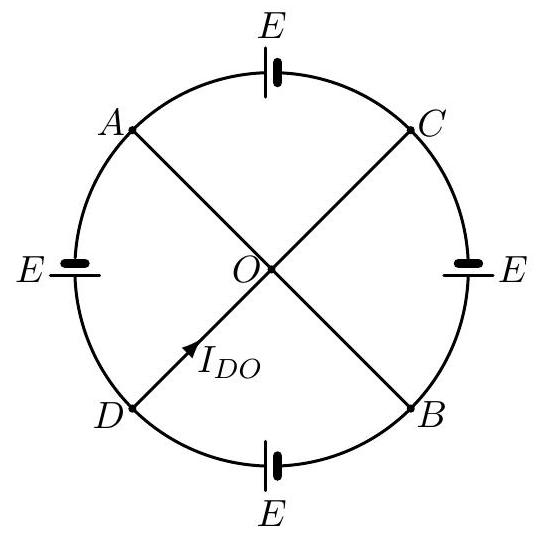
\includegraphics[width=0.4\linewidth]{images/2025_08_19_9e83650bd9c853eca85eg-04(1)}\\ Notăm $R$ rezistenţa electrică a unui fir conductor de lungime egală cu raza cercului.\\ $R=0,1 \frac{\Omega}{\mathrm{~m}} \cdot 1 \mathrm{~m}=0,1 \Omega$.\\ Să observăm că circuitul electric este simetric în raport cu diametrul $C D$. În baza acestei proprietăţi, prin laturile $O A$ şi $O B$ trec curenţi egali, ambii intrând în $O$ sau ambii ieşind din $O$. Conform primei teoreme a lui Kirchhoff aplicată nodului $O$, prin latura $O C$ trece un curent egal cu $I_{D O}$, de la $O$ la $C$. În $C$, din motive de simetrie, acest curent se desparte în părţi egale, $I_{D O} / 2$ care circulă de la $C$ la $A$, respectiv de la $C$ la $B$. Considerând nodul $D$, justificăm similar trecerea unui curent $I_{D O} / 2$ de la $A$ la $D$ şi de la $B$ la $D$. Aplicăm acum prima teoremă a lui Kirchhoff nodurilor $A$ şi $B$ obţinând că prin laturile $O A$ şi $O B$ nu trece curent electric. Laturile $O A$ şi $O B$ pot fi scoase din circuit fără a afecta comportarea electrică a acestuia. Schema electrică echivalentă este prezentată mai jos.\\ \begin{center} 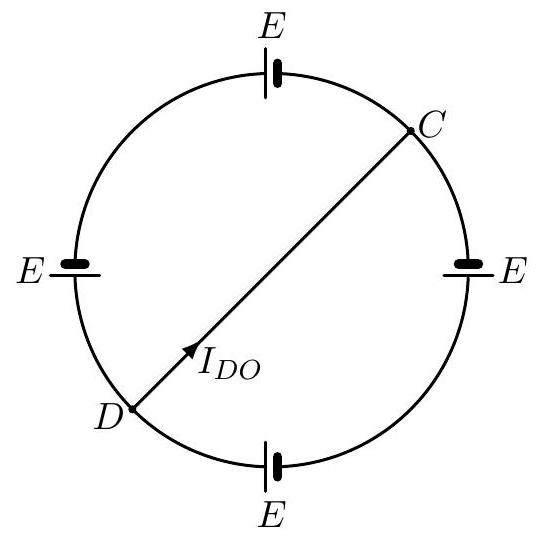
\includegraphics[width=0.4\linewidth]{images/2025_08_19_9e83650bd9c853eca85eg-04} \end{center}\\ Fiecare semicerc se comportă ca o sursă cu t.e.m. $2 E$ şi rezistenţa internă $\pi R$. Montajul paralel al acestor surse identice este echivalent cu o singură sursă cu t.e.m. $2 E$ şi rezistenţa internă $\pi R / 2$. Această sursă echivalentă alimentează consumatorul cu rezistenţa electrică $2 R$ a diametrului $C D$.\\ $I_{D O}=\frac{2 E}{2 R+\pi R / 2}=\frac{4}{4+\pi} \frac{E}{R}=\frac{4}{4+\pi} \frac{1 \mathrm{~V}}{0,1 \Omega}=\frac{40}{4+\pi} \mathrm{A}$.\\

2014.A.12. Două rezistoare cu rezistenţele $R_{1}=0,5 \Omega$ şi $R_{2}=0,75 \Omega$ sunt montate în serie, iar gruparea este conectată la o sursă cu t.e.m. de $5,4 \mathrm{~V}$ şi rezistenţa internă de $0,1 \Omega$. Puterea disipată pe rezistorul $R_{1}$ este: (5 pct.)\\ a) $2,25 \mathrm{~W}$; b) $2 \mathrm{~W}$; c) $16 \mathrm{~W}$; d) $8 \mathrm{~W}$; e) $2,25 \mathrm{~W}$; f) $4 \mathrm{~W}$.\\ Notăm $E=5,4 \mathrm{~V}$ şi $r=0,1 \Omega$. Curentul în circuit este $I=E /\left(R_{1}+R_{2}+r\right)$, iar puterea disipată pe rezistorul $R_{1}$ este:\\ $I^{2} R_{1}=\frac{E^{2} R_{1}}{\left(R_{1}+R_{2}+r\right)^{2}}=8 \mathrm{~W}$.\\

2014.A.13. Considerând ciclurile termodinamice Carnot, Otto şi Diesel, două transformări izocore apar în: (5 pct.)\\ a) în toate trei; b) ciclul Diesel; c) ciclul Carnot; d) în niciunul; e) în ciclurile Carnot şi Diesel; f) ciclul Otto.\\ Ciclul Otto.\\

2014.A.14. Un mobil pleacă din repaus şi în primele $n$ secunde parcurge rectiliniu uniform accelerat un spaţiu egal cu $2 n^{2}$ metri. Acceleraţia mobilului este egală cu: (5 pct.)\\ a) $2 \mathrm{~m} / \mathrm{s}^{2}$; b) $4 \mathrm{~m} / \mathrm{s}^{2}$; c) $2,25 \mathrm{~m} / \mathrm{s}^{2}$; d) $8 \mathrm{~m} / \mathrm{s}^{2}$; e) $10 \mathrm{~m} / \mathrm{s}^{2}$; f) $1 \mathrm{~m} / \mathrm{s}^{2}$.\\ Notăm $t=n \mathrm{~s}$ şi $d=2 n^{2} \mathrm{~m}$. Din ecuaţia de mişcare $d=\frac{1}{2} a t^{2}$, acceleraţia mişcării este: $a=\frac{2 d}{t^{2}}=4 \mathrm{~m} / \mathrm{s}^{2}$.\\

2014.A.15. Sub acţiunea unei forţe orizontale de $50 \mathrm{~N}$, un corp se deplasează orizontal timp de $2 \mathrm{~min}$ cu viteza constantă de $5 \mathrm{~m} / \mathrm{s}$. Lucrul mecanic efectuat de forţă este: (5 pct.)\\ a) $2500 \mathrm{~J}$; b) $180 \mathrm{~N} \cdot \mathrm{~m}$; c) $30 \mathrm{~J}$; d) $8 \mathrm{~kJ}$; e) $30 \mathrm{~kJ}$; f) $1000 \mathrm{~J}$.\\ Notăm $F=50 \mathrm{~N}$, $\Delta t=2 \mathrm{~min}=120 \mathrm{~s}$ şi $v=5 \mathrm{~m} / \mathrm{s}$. Distanţa străbătută de corp este $d=v \Delta t$.\\ Lucrul mecanic efectuat de forţă este $F d=F v \Delta t=30000 \mathrm{~J}=30 \mathrm{~kJ}$.\\

2014.A.16. Impulsul unui corp este $4 \mathrm{~kg} \cdot \mathrm{~m} / \mathrm{s}$, iar energia sa cinetică este $16 \mathrm{~J}$. Masa corpului este: (5 pct.)\\ a) $2 \mathrm{~kg}$; b) $0,5 \mathrm{~kg}$; c) $1,5 \mathrm{~kg}$; d) $0,1 \mathrm{~kg}$; e) $0,75 \mathrm{~kg}$; f) $1 \mathrm{~kg}$.\\ Notăm $p=4 \mathrm{~kg} \cdot \mathrm{~m} / \mathrm{s}$, $E_{\mathrm{c}}=16 \mathrm{~J}$, $m$ - masa corpului şi $v$ - viteza acestuia.\\ Între relaţiile de definiţie $p=m v$ şi $E_{\mathrm{c}}=(1 / 2) m v^{2}$ eliminăm $v$.\\ Se obţine: $m=\frac{p^{2}}{2 E_{\mathrm{c}}}=0,5 \mathrm{~kg}$.\\

2014.A.17. Un volum de $30$ litri dintr-un gaz ideal aflat la presiunea de $16,62 \cdot 10^{5} \mathrm{~N} / \mathrm{m}^{2}$ şi temperatura de $300 \mathrm{~K}$ ($R=8,31 \mathrm{~J} / \mathrm{mol} \mathrm{K}$) conţine un număr de moli egal cu: (5 pct.)\\ a) $20$; b) $1$; c) $15$; d) $14$; e) $30$; f) $2$.\\ Notăm $V=30 \mathrm{~L}=3 \cdot 10^{-2} \mathrm{~m}^{3}$, $p=16,62 \cdot 10^{5} \mathrm{~N} / \mathrm{m}^{2}$, $T=300 \mathrm{~K}$ şi $\nu$ - cantitatea de gaz.\\ Din ecuaţia termică de stare a gazului ideal $p V=\nu R T$ rezultă:\\ $\nu=\frac{p V}{R T}=20 \mathrm{~mol}$.\\

2014.A.18. În Arctica iarna, temperatura aerului atinge $-37,36^{\circ} \mathrm{C}$, în timp ce temperatura apei sub gheaţă este $+1^{\circ} \mathrm{C}\left(0^{\circ} \mathrm{C}=273 \mathrm{~K}\right)$. O maşină bitermă ideală care lucrează între aceste temperaturi are randamentul: (5 pct.)\\ a) $30 \%$; b) $5 \%$; c) $14 \%$; d) $50 \%$; e) $10 \%$; f) $1 \%$.\\ Temperatura sursei calde este $T_{1}=(273+1) \mathrm{K}=274 \mathrm{~K}$ şi temperatura sursei reci este $T_{2}=(273-37,36) \mathrm{K}=235,64 \mathrm{~K}$. Randamentul maşinii termice este:\\ $\eta=\frac{T_{1}-T_{2}}{T_{1}}=0,14=14 \%$.\\

% iulie 2013, Admitere UPB, Fizică F. Enunțuri şi rezolvare %

2013.A.1. Un conductor de cupru ($\rho=1,7 \cdot 10^{-8} \Omega \cdot \mathrm{m}$) are lungimea de $300 \mathrm{~m}$ şi aria secţiunii transversale de $1 \mathrm{~mm}^{2}$. Rezistenţa conductorului este:\\ a) $10,1 \Omega$; b) $2,2 \Omega$; c) $3,5 \Omega$; d) $5,1 \Omega$; e) $7,5 \Omega$; f) $4,7 \Omega$.\\ Rezistenţa conductorului este $R=\rho \frac{l}{S}=5,1 \Omega$.\\

2013.A.2. Un gaz ideal suferă o transformare izobară la presiunea de $10^{5} \mathrm{~N} / \mathrm{m}^{2}$ în cursul căreia volumul său creşte de la $10 \mathrm{dm}^{3}$ la $50 \mathrm{dm}^{3}$. Lucrul mecanic efectuat de gaz este:\\ a) $4 \mathrm{~kJ}$; b) $4 \cdot 10^{6} \mathrm{~J}$; c) $8 \mathrm{~kJ}$; d) $1,2 \mathrm{~kJ}$; e) $400 \mathrm{~J}$; f) $5 \mathrm{~J}$.\\ Lucrul mecanic efectuat de gaz într-o transformare izobară este:\\ $L=p \Delta V=4 \mathrm{~kJ}$.\\

2013.A.3. Un motor termic funcţionează după un ciclu Carnot cu randamentul $0,5$. Cunoscând temperatura sursei reci de $250 \mathrm{~K}$, temperatura sursei calde este:\\ a) $600 \mathrm{~K}$; b) $500 \mathrm{~K}$; c) $800 \mathrm{~K}$; d) $400 \mathrm{~K}$; e) $1000 \mathrm{~K}$; f) $300 \mathrm{~K}$.\\ Din randamentul ciclului Carnot $\eta=1-\frac{T_{2}}{T_{1}}$, rezultă temperatura sursei calde:\\ $T_{1}=500 \mathrm{~K}$.\\

2013.A.4. La bornele unui acumulator cu t.e.m. de $10 \mathrm{~V}$ și rezistenţa internă de $1 \Omega$ se leagă un rezistor cu rezistenţa de $4 \Omega$. Puterea disipată pe rezistor este:\\ a) $4 \mathrm{~W}$; b) $64 \mathrm{~W}$; c) $8 \mathrm{~W}$; d) $16 \mathrm{~W}$; e) $32 \mathrm{~W}$; f) $20 \mathrm{~W}$.\\ Puterea disipată pe rezistor este: $P=\frac{R E^{2}}{(R+r)^{2}}=16 \mathrm{~W}$.\\

2013.A.5. Un corp cu masa de $10 \mathrm{kg}$ este tras pe un plan orizontal cu o forţă de $70 \mathrm{~N}$ paralelă cu planul. În absenţa frecărilor, acceleraţia corpului este:\\ a) $0,14 \mathrm{~m} / \mathrm{s}^{2}$; b) $21 \mathrm{~m} / \mathrm{s}^{2}$; c) $700 \mathrm{~m} / \mathrm{s}^{2}$; d) $7 \mathrm{~m} / \mathrm{s}^{2}$; e) $5 \mathrm{~m} / \mathrm{s}^{2}$; f) $0,17 \mathrm{~m} / \mathrm{s}^{2}$.\\ Din $\vec{F}=m \vec{a}$ rezultă $a=7 \mathrm{~m} / \mathrm{s}^{2}$.\\

2013.A.6. Un corp de masă $2 \mathrm{~kg}$ se deplasează cu viteza de $15 \mathrm{~m} / \mathrm{s}$. Impulsul corpului este:\\ a) $17 \mathrm{~kg} \cdot \mathrm{~m} / \mathrm{s}$; b) $30 \mathrm{~kg} \cdot \mathrm{~m} / \mathrm{s}$; c) $7,5 \mathrm{~kg} \cdot \mathrm{~m} / \mathrm{s}$; d) $225 \mathrm{~J}$; e) $225 \mathrm{~kg} \cdot \mathrm{~m} / \mathrm{s}$; f) $15 \mathrm{~N}$.\\ Impulsul corpului este: $\vec{p}=m \vec{v}=30 \mathrm{~kg} \cdot \mathrm{~m} / \mathrm{s}$.\\

2013.A.7. În SI puterea se măsoară în: a) $\frac{\mathrm{kW}}{\mathrm{h}}$; b) $\mathrm{J} \cdot \mathrm{s}$; c) $\mathrm{kg} \cdot \mathrm{s}$; d) $\mathrm{kWh}$; e) $\mathrm{N} \cdot \mathrm{m}$; f) $\mathrm{W}$.\\ În SI puterea se măsoară în Wați ($\mathrm{W}$).\\

2013.A.8. Volumul unui gaz ideal a fost redus izoterm cu $20 \%$. Presiunea gazului a crescut cu:\\ a) $20 \%$; b) $22,5 \%$; c) $12 \%$; d) $33 \%$; e) $18 \%$; f) $25 \%$.\\ Din ecuaţia transformării izoterme $p V=$ const., rezultă:\\ $p_{1} V_{1}=\left(p_{1}+x p_{1}\right) \cdot\left(V_{1}-f V_{1}\right)$;\\ Deci $x=25 \%$.\\

2013.A.9. Secţiunea transversală a unui conductor este traversată în $3 \mathrm{~s}$ de o sarcină electrică de $1,8 \mathrm{C}$. Intensitatea curentului prin conductor este:\\ a) $0,8 \mathrm{~A}$; b) $5,4 \mathrm{~A}$; c) $6 \mathrm{~A}$; d) $1 \mathrm{~A}$; e) $0,54 \mathrm{~A}$; f) $0,6 \mathrm{~A}$.\\ Intensitatea curentului prin conductor este: $I=\frac{q}{\Delta t}=0,6 \mathrm{~A}$.\\

2013.A.10. Un gaz ideal aflat într-un recipient de volum $6 \mathrm{dm}^{3}$ are presiunea de $16,62 \cdot 10^{5} \mathrm{~N} / \mathrm{m}^{2}$ la temperatura de $300 \mathrm{~K}$ . Dacă $R=8,31 \mathrm{~J} / \mathrm{mol} \cdot \mathrm{K}$, numărul de moli de gaz este:\\ a) $6$; b) $4$; c) $16$; d) $2$; e) $8$; f) $1$.\\ Din ecuaţia de stare a gazului ideal, $p V=\nu R T$, rezultă numărul de moli de gaz: $\nu=4$ moli.\\

2013.A.11. Trei rezistori cu rezistenţele de $5 \Omega$, $6 \Omega$, $14 \Omega$ sunt legaţi în serie. Rezistenţa echivalentă a grupării este:\\ a) $13 \Omega$; b) $3 \Omega$; c) $11 \Omega$; d) $25 \Omega$; e) $35 \Omega$; f) $15 \Omega$.\\ Rezistenţa echivalentă a grupării de rezistoare legate în serie este:\\ $R_{e}=R_{1}+R_{2}+R_{3}=25 \Omega$.\\

2013.A.12. Un automobil cu masa de $900 \mathrm{~kg}$ are energia cinetică de $180 \mathrm{~kJ}$ . Viteza automobilului este:\\ a) $15 \mathrm{~m} / \mathrm{s}$; b) $10 \mathrm{~m} / \mathrm{s}$; c) $24 \mathrm{~m} / \mathrm{s}$; d) $20 \mathrm{~m} / \mathrm{s}$; e) $2 \mathrm{~m} / \mathrm{s}$; f) $400 \mathrm{~m} / \mathrm{s}$.\\ Din expresia energiei cinetice, $E_{c}=\frac{m v^{2}}{2}$, rezultă viteza automobilului:\\ $v=20 \mathrm{~m} / \mathrm{s}$.\\

2013.A.13. O baterie formată din patru elemente identice legate în serie, fiecare element având t.e.m. de $2,5 \mathrm{~V}$ şi rezistenţa internă de $0,1 \Omega$, alimentează un circuit format din două rezistoare cu rezistențele $R_{1}=16 \Omega$ și $R_{2}=24 \Omega$ legate în paralel. Energia disipată pe rezistorul $R_{1}$ în timp de $1000 \mathrm{~s}$ este:\\ a) $2130 \mathrm{~J}$; b) $8200 \mathrm{~J}$; c) $5,76 \mathrm{~J}$; d) $2,84 \mathrm{~kJ}$; e) $5,76 \mathrm{~kJ}$; f) $4580 \mathrm{~J}$.\\ Intensitatea curentului în circuitul format din baterie și rezistenţa echivalentă grupării de rezistoare legate în paralel este: $I=\frac{n E}{n r+\frac{R_{1} R_{2}}{R_{1}+R_{2}}}$. Acest curent se împarte între cele două rezistoare astfel încât: $I=I_{1}+I_{2}$ şi $I_{1} R_{1}=I_{2} R_{2}$, de unde rezultă $I_{1}=\frac{I R_{2}}{R_{1}+R_{2}}$.\\ Energia disipată pe rezistorul $R_{1}$ în timpul $t$ este: $W_{1}=R_{1} I_{1}^{2} t=5,76 \mathrm{~kJ}$.\\

2013.A.14. Un generator cu t.e.m. de $12 \mathrm{~V}$ are intensitatea curentului de scurtcircuit de $40 \mathrm{~A}$. Rezistenţa unui rezistor, care legat la bornele generatorului face ca tensiunea la borne să fie egală cu $11 \mathrm{~V}$, este:\\ a) $3,3 \Omega$; b) $1,4 \Omega$; c) $3 \Omega$; d) $2,8 \Omega$; e) $6,2 \Omega$; f) $3,6 \Omega$.\\ Tensiunea la bornele rezistorului este: $U=\frac{R E}{R+\frac{E}{I_{s}}}$, de unde $R=3,3 \Omega$.\\

2013.A.15. Un corp cu masa de $50 \mathrm{~kg}$ este ridicat vertical cu viteza de $3 \mathrm{~m} / \mathrm{s}$ timp de $8 \mathrm{~s}$ ($g=10 \mathrm{~m} / \mathrm{s}^{2}$) folosind un motor termic cu randamentul de $60 \%$. Valoarea absolută a căldurii cedate de motor este:\\ a) $2 \mathrm{~kJ}$; b) $10 \mathrm{~kJ}$; c) $8 \mathrm{~kJ}$; d) $3,2 \mathrm{~kJ}$; e) $4 \mathrm{~kJ}$; f) $240 \mathrm{~J}$.\\ Randamentul motorului este $\eta=\frac{L}{Q_{p}}$ iar $L=Q_{p}-\left|Q_{c}\right|$, de unde rezultă:\\ $\left|Q_{c}\right|=L\left(\frac{1}{\eta}-1\right)=\mathrm{m g v t}\left(\frac{1}{\eta}-1\right)=8 \mathrm{~kJ}$.\\

2013.A.16. Un automobil electric cu masa de $0,4 \mathrm{t}$ coboară o pantă cu viteza constantă de $18 \mathrm{~km} / \mathrm{h}$ ($g=10 \mathrm{~m} / \mathrm{s}^{2}$) cu motorul oprit. La urcarea pantei cu aceeaşi viteză, motorul automobilului consumă un curent de $50 \mathrm{~A}$ la tensiunea de $100 \mathrm{~V}$. Sinusul unghiului format de pantă cu orizontala este:\\ a) $\frac{1}{2}$; b) $\frac{1}{8}$; c) $\frac{\sqrt{2}}{2}$; d) $0,3$; e) $\frac{\sqrt{3}}{2}$; f) $\frac{1}{16}$.\\ Ecuaţiile de mişcare la coborârea şi urcarea pantei cu viteză constantă sunt: $m g \sin \alpha-\mu m g \cos \alpha=0$ şi respectiv $F-m g \sin \alpha-\mu m g \cos \alpha=0$ în care $F$ este forţa motorului: $F=\frac{U I}{v}$. Rezultă $\sin \alpha=\frac{1}{8}$.\\

2013.A.17. O cantitate de gaz ideal monoatomic ($C_{V}=\frac{3}{2} R$) parcurge ciclul reversibil din figură. Randamentul ciclului este:\\ a) $0,18$; b) $0,25$; c) $\frac{16}{97}$; d) $\frac{1}{6}$; e) $0,07$; f) $\frac{1}{7}$.\\ 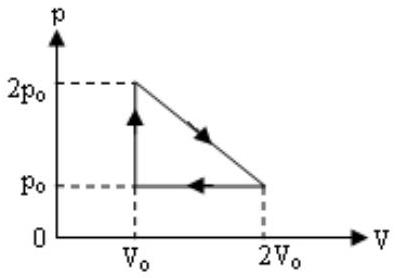
\includegraphics[width=0.4\linewidth]{images/2025_08_19_9e83650bd9c853eca85eg-10}\\ Randamentul ciclului este $\eta=\frac{L}{Q_{p}}$.\\ Lucrul mecanic efectuat de gaz într-un ciclu este $L=\frac{p_{0} V_{0}}{2}$.\\ \begin{center} 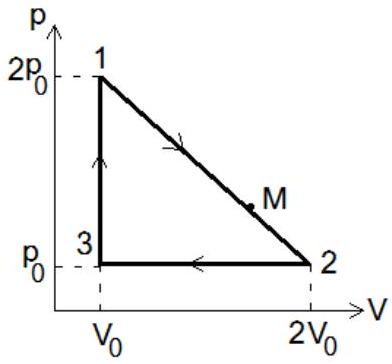
\includegraphics[width=0.4\linewidth]{images/2025_08_19_9e83650bd9c853eca85eg-10(1)} \end{center}\\ Gazul primeşte căldură în transformarea izocoră $Q_{31}=\nu C_{V}\left(T_{1}-T_{3}\right)=\frac{3}{2} p_{0} V_{0}$ şi pe porţiunea 1-M din transformarea $1-2$, $Q_{1 M}$, care se calculează în felul următor:\\ Ecuaţia dreptei $1-2$ este $p=a V+b$ cu $a=-\frac{p_{0}}{V_{0}}$ şi $b=3 p_{0}$;\\ Considerând un punct oarecare (de coordonate $p, V$ ) de pe dreapta $1-2$, se calculează lucrul mecanic, variaţia de energie internă şi căldura pe transformarea 1-acel punct:\\ $L(V)=\frac{\left(p+2 p_{0}\right)\left(V-V_{0}\right)}{2}=-\frac{p_{0} V^{2}}{2 V_{0}}+3 p_{0} V-\frac{5 p_{0} V_{0}}{2}$\\ $\Delta U(V)=\nu C_{V}\left(T-T_{1}\right)=-\frac{3 p_{0} V^{2}}{2 V_{0}}+\frac{9 p_{0} V}{2}-3 p_{0} V_{0}$\\ $Q(V)=\Delta U(V)+L(V)=-\frac{2 p_{0} V^{2}}{V_{0}}+\frac{15 p_{0} V}{2}-\frac{11 p_{0} V_{0}}{2}$.\\ Din condiţia ca funcţia $Q(V)$ să prezinte un maxim, $Q^{\prime}(V)=0$, rezultă volumul corespunzător punctului $\mathrm{M}$, $V_{M}=\frac{15}{8} V_{0}$, şi căldura $Q_{1 M}=\frac{49}{32} p_{0} V_{0}$.\\ Căldura totală primită de gaz pe un ciclu este $Q_{p}=Q_{31}+Q_{1 M}=\frac{97}{32} p_{0} V_{0}$, iar randamentul ciclului are valoarea $\eta=\frac{16}{97}$.\\

2013.A.18. Un corp cade liber. În secunda $n$ a mişcării corpul parcurge o distanţă de $1,4$ ori mai mare decât în secunda anterioară. Dacă se neglijează frecarea cu aerul, valoarea lui $n$ este:\\ a) $4$; b) $2$; c) $5$; d) $7$; e) $8$; f) $3$.\\ Spaţiile parcurse de corp în primele $n$, $n-1$ și respectiv $n-2$ secunde sunt: $s_{n}=\frac{1}{2} g n^{2}$, $s_{n-1}=\frac{1}{2} g(n-1)^{2}$, $s_{n-2}=\frac{1}{2} g(n-2)^{2}$.\\ Din condiţia $s_{n}-s_{n-1}=k\left(s_{n-1}-s_{n-2}\right)$, cu $k=1,4$, rezultă $n=4$.\\

% iulie 2012, Admitere UPB, Fizică F. Enunțuri şi rezolvare %

2012.A.1. Două rezistoare cu rezistențele $R_{1}=4 \Omega$ şi $R_{2}=8 \Omega$ se montează în serie, apoi în paralel. Raportul dintre rezistențele echivalente serie/paralel este:\\ a) $1 / 2$; b) $9 / 2$; c) $2$; d) $3 / 16$; e) $2 / 9$; f) $16 / 3$.\\ Rezistenţele echivalente serie, respectiv paralel, sunt:\\ $R_{s}=R_{1}+R_{2}$ şi $R_{p}=\frac{R_{1} R_{2}}{R_{1}+R_{2}}$.\\ Raportul lor este: $\frac{R_{s}}{R_{p}}=\frac{\left(R_{1}+R_{2}\right)^{2}}{R_{1} R_{2}}=\frac{9}{2}$.\\

2012.A.2. Conductoarele $\mathrm{AB}$, $\mathrm{BC}$, $\mathrm{CD}$ și $\mathrm{DA}$ formează un circuit dreptunghiular ca în figură, iar conductorul $\mathrm{AC}$ este pe diagonală. Toate conductoarele au aceeaşi rezistenţă pe unitatea de lungime. Laturile dreptunghiului au lungimile $a$ şi $b=\frac{4 a}{3}$. Rezistenţa echivalentă între punctele B şi D se notează cu $R_{B D}$, iar cea între punctele A şi C cu $R_{A C}$. Raportul dintre $R_{B D}$ şi $R_{A C}$ este:\\ a) $27 / 35$; b) $24 / 35$; c) $48 / 35$; d) $79 / 35$; e) $62 / 35$; f) $59 / 35$.\\ 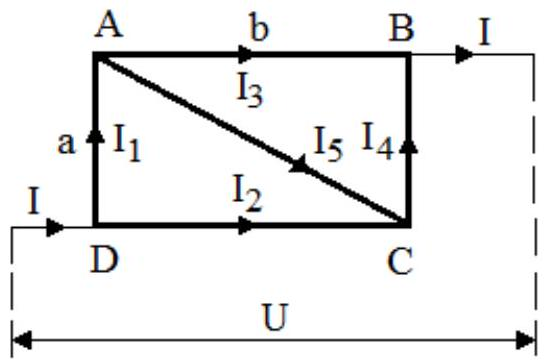
\includegraphics[width=0.4\linewidth]{images/2025_08_19_9e83650bd9c853eca85eg-12}\\ Figura problemei:\\ \begin{center} 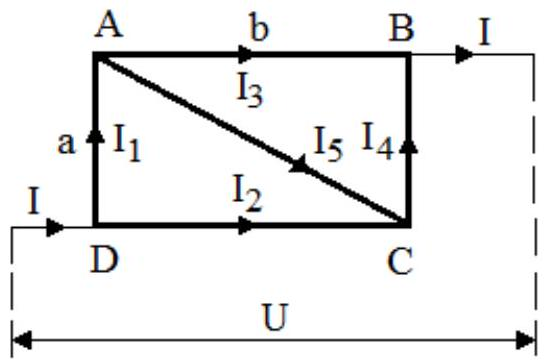
\includegraphics[width=0.4\linewidth]{images/2025_08_19_9e83650bd9c853eca85eg-12} \end{center}\\ Dacă notăm cu $\beta$ rezistenţa pe unitatea de lungime a conductoarelor, atunci rezistențele laturilor dreptunghiului sunt:\\ $r_{A B}=\frac{4}{3} \beta a$, $r_{B C}=\beta a$, $r_{C D}=\frac{4}{3} \beta a$, $r_{A D}=\beta a, r_{A C}=\frac{5}{3} \beta a$.\\ Rezistenţa echivalentă între punctele A şi C, $R_{A C}$, are valoarea:\\ $R_{A C}=\frac{1}{1 /\left(r_{A B}+r_{B C}\right)+1 /\left(r_{A D}+r_{C D}\right)+1 / r_{A C}}=\frac{35}{51} \beta a$.\\ Rezistenţa echivalentă între punctele B și D se calculează considerând situaţia în care puntea este alimentată între aceste două puncte la tensiunea $U$ şi prin conductoare circulă curenţi electrici, notaţi ca în figură. Considerând tensiunea un parametru fixat, din rezolvarea sistemului de 5 ecuaţii cu 5 necunoscute (curenţii $I$), sistem obţinut din legile lui Kirchhoff:\\ $I_{1}-I_{3}-I_{5}=0; \quad I_{2}+I_{5}-I_{4}=0; \quad \beta a I_{1}+\frac{5 \beta a}{3} I_{5}-\frac{4 \beta a}{3} I_{2}=0; \quad \beta a I_{1}+\frac{4 \beta a}{3} I_{3}=U; \quad \frac{4 \beta a}{3} I_{2}+\beta a I_{4}=U$\\ Rezultă $I_{1}=\frac{27}{59 \beta a} U$ şi $I_{2}=\frac{24}{59 \beta a} U$. Deoarece $I=I_{1}+I_{2}$ şi $R_{B D}=\frac{U}{I}$, obţinem $R_{B D}=\frac{59}{51} \beta a$ şi raportul $\frac{R_{B D}}{R_{A C}}=\frac{59}{35}$.\\

2012.A.3. Pornind fără viteză iniţială, un mobil se deplasează rectiliniu pe distanţa de $100 \mathrm{~m}$. Pe primul şi ultimul sfert din distanţa parcursă mobilul se mişcă cu aceeaşi acceleraţie constantă, iar în rest viteza sa este constantă şi egală cu $10 \mathrm{~m} / \mathrm{s}$. Durata deplasării este:\\ a) $5(\sqrt{2}+1) \mathrm{s}$; b) $5 \sqrt{2} \mathrm{~s}$; c) $0,01 \mathrm{~h}$; d) $5(\sqrt{2}-1) \mathrm{s}$; e) $14 \mathrm{~s}$; f) $5 / \sqrt{2} \mathrm{~s}$.\\ Pentru primul sfert de drum, din formula lui Galilei, $v^{2}=2 a \frac{d}{4}$, se obţine acceleraţia $a$. Astfel, durata deplasării pe primul sfert de drum este:\\ $t_{1}=\frac{v}{a}=\frac{d}{2 v}=5 \mathrm{~s}$.\\ Durata în care mobilul se deplasează cu viteză constantă este:\\ $t_{2}=\frac{d}{2 v}=5 \mathrm{~s}$.\\ După parcurgerea ultimului sfert de drum, viteza finală este $v_{f}=\sqrt{v^{2}+2 a \frac{d}{4}}$, iar durata corespunzătoare este $t_{3}=\frac{v_{f}-v}{a}=5(\sqrt{2}-1) \mathrm{s}$.\\ Durata totală a deplasării este $t=t_{1}+t_{2}+t_{3}=5(\sqrt{2}+1) \mathrm{s}$.\\

2012.A.4. Două automobile pleacă în acelaşi moment unul spre celălalt din două localităţi aflate la distanţa de $120 \mathrm{~km}$. Vehiculele se deplasează cu aceeaşi viteză constantă de $60 \mathrm{~km} / \mathrm{h}$. Mobilele se întâlnesc după:\\ a) $1,5 \mathrm{~h}$; b) $2 \mathrm{~h}$; c) $75$ minute; d) $60$ minute; e) $45$ minute; f) $3 \mathrm{~h}$.\\ Din condiţia de întâlnire, $d=v_{1} t+v_{2} t$, rezultă $t=60$ minute.\\

2012.A.5. Un corp cu masa de $100 \mathrm{~kg}$ se află la $10 \mathrm{~m}$ deasupra solului. Se consideră $g=9,81 \mathrm{~m} \cdot \mathrm{~s}^{-2}$. Energia potenţială gravitaţională a corpului este:\\ a) $981 \mathrm{~J}$; b) $9,81 \mathrm{~J}$; c) $1 \mathrm{~kJ}$; d) $98,10 \mathrm{~J}$; e) $9810 \mathrm{~J}$; f) $98,1 \mathrm{~kJ}$.\\ Energia potenţială gravitaţională a corpului este: $E_{p}=m g h=9810 \mathrm{~J}$.\\

2012.A.6. Căldura degajată la trecerea unui curent electric de intensitate $I$ printr-un conductor de rezistenţă $R$, în intervalul de timp $\Delta t$ este:\\ a) $I^{2} R \Delta t$; b) $I R^{2} \Delta t^{2}$; c) $I R^{2} \Delta t$; d) $I / R^{2} \Delta t$; e) $I^{2} R^{2} / \Delta t$; f) $I^{2} R^{2} \Delta t$.\\ Căldura degajată este: $Q=R I^{2} \Delta t$.\\

2012.A.7. Un circuit electric simplu este format dintr-o sursă de tensiune cu rezistenţa internă $r$ şi un rezistor cu rezistenţa $R=4 r$. Randamentul circuitului este:\\ a) $0,2$; b) $0,3$; c) $0,7$; d) $0,4$; e) $0,6$; f) $0,8$.\\ Randamentul circuitului electric este: $\eta=\frac{P_{u}}{P_{c}}=\frac{R}{R+r}=0,8$.\\

2012.A.8. Randamentul unui ciclu Carnot care funcţionează între temperaturile $T_{1}=600 \mathrm{~K}$ şi $T_{2}=300 \mathrm{~K}$ este:\\ a) $0,4$; b) $0,6$; c) $0,75$; d) $0,5$; e) $0,25$; f) $0,55$.\\ Randamentul ciclului Carnot este: $\eta=1-\frac{T_{2}}{T_{1}}=0,5$.\\

2012.A.9. Relaţia Robert-Mayer este:\\ a) $C_{p}=C_{V}+R$; b) $\gamma=C_{p} / C_{V}$; c) $C_{V}=C_{p}+R$; d) $C_{p}=C_{V}-R / 2$; e) $R=C_{p}+C_{V}$; f) $\Delta U=Q-L$.\\ Relaţia Robert-Mayer este: $C_{p}=C_{V}+R$.\\

2012.A.10. Expresia legii lui Ohm pentru un circuit simplu este:\\ a) $I=\frac{U}{R}+\frac{E}{r}$; b) $I=\frac{U}{R}$; c) $I=\frac{E}{r}$; d) $I=\frac{U}{r}$; e) $I=\frac{E}{R+r}$; f) $I=\frac{U}{R+r}$.\\ Legea lui Ohm pentru un circuit simplu este: $I=\frac{E}{R+r}$.\\

2012.A.11. Unitatea de măsură în SI pentru rezistivitatea electrică a unui material conductor este:\\ a) $\Omega$; b) $\Omega \cdot \mathrm{m}^{2}$; c) $\frac{\Omega}{\mathrm{m}}$; d) $\frac{\Omega^{2}}{\mathrm{m}}$; e) $\Omega \cdot \mathrm{m}$; f) $\Omega^{2} \cdot \mathrm{m}$.\\ $[\rho]_{S I}=\Omega \cdot \mathrm{m}$.\\

2012.A.12. În condiţii normale de presiune şi temperatură $\left(p_{0}, T_{0}\right)$, densitatea unui gaz ideal este $\rho_{0}$. Cunoscând căldura specifică a gazului la volum constant $c_{V}$, exponentul său adiabatic este:\\ a) $\frac{\rho_{0}}{p_{0} T_{0} c_{V}}$; b) $1+\frac{\rho_{0}}{p_{0} c_{V}}$; c) $\frac{p_{0}}{\rho_{0} T_{0} c_{V}}$; d) $1+\frac{\rho_{0} T_{0} c_{V}}{p_{0}}$; e) $1-\frac{\rho_{0} T_{0} c_{V}}{p_{0}}$; f) $1+\frac{p_{0}}{\rho_{0} T_{0} c_{V}}$.\\ $\gamma=\frac{C_{p}}{C_{V}}=\frac{C_{V}+R}{C_{V}}=1+\frac{R}{C_{V}}=1+\frac{R}{\mu C_{V}}$. Din ecuaţia termică de stare, $p_{0} V_{0}=\frac{m}{\mu} R T_{0}$, rezultă $\frac{R}{\mu}=\frac{p_{0} V_{0}}{m T_{0}}=\frac{p_{0}}{\rho_{0} T_{0}}$. Înlocuind în expresia lui $\gamma$ rezultă $\gamma=1+\frac{p_{0}}{\rho_{0} T_{0} c_{V}}$.\\

2012.A.13. În cursul unui ciclu termodinamic cu randamentul $\eta=0,2$ se efectuează un lucru mecanic de $1000 \mathrm{~J}$. Căldura cedată sursei reci în cursul ciclului are valoarea absolută de:\\ a) $5 \mathrm{~kJ}$; b) $1 \mathrm{~kJ}$; c) $6000 \mathrm{~J}$; d) $4 \mathrm{~kJ}$; e) $2000 \mathrm{~J}$; f) $3 \mathrm{~kJ}$.\\ Din expresia randamentului, $\eta=\frac{L}{Q_{p}}$, se obţine căldura primită, $Q_{p}$, iar din expresia lucrului mecanic, $L=Q_{p}-\left|Q_{c}\right|$, rezultă $\left|Q_{c}\right|=\frac{L}{\eta}-L=4 \mathrm{~kJ}$.\\

2012.A.14. Un sistem termodinamic primeşte căldura $Q=400 \mathrm{~J}$ şi efectuează lucrul mecanic $L=200 \mathrm{~J}$. Variaţia energiei sale interne este:\\ a) $400 \mathrm{~J}$; b) -$200 \mathrm{~J}$; c) $1000 \mathrm{~J}$; d) $800 \mathrm{~J}$; e) $200 \mathrm{~J}$; f) $600 \mathrm{~J}$.\\ Din ecuaţia principiului I al termodinamicii, $Q=\Delta U+L$, rezultă:\\ $\Delta U=Q-L=200 \mathrm{~J}$.\\

2012.A.15. Sub acţiunea unei forţe de $10 \mathrm{~kN}$ o bară metalică nedeformată se alungeşte cu $40 \mathrm{~mm}$. Lucrul mecanic efectuat este:\\ a) $120 \mathrm{~J}$; b) $350 \mathrm{~J}$; c) $50 \mathrm{~J}$; d) $970 \mathrm{~J}$; e) $80 \mathrm{~J}$; f) $200 \mathrm{~J}$.\\ Forţa deformatoare este $F=k x$. Lucrul mecanic efectuat de această forţă este:\\ $L=\frac{k x^{2}}{2}=\frac{F x}{2}=200 \mathrm{~J}$.\\

2012.A.16. Un mobil se deplasează rectiliniu cu viteza constantă de $84 \frac{\mathrm{km}}{\mathrm{h}}$. Distanţa parcursă de mobil în $1200 \mathrm{~s}$ este:\\ a) $100 \mathrm{~m}$; b) $68 \mathrm{~km}$; c) $77 \mathrm{~m}$; d) $76 \mathrm{~km}$; e) $50 \mathrm{~m}$; f) $28 \mathrm{~km}$.\\ Distanţa parcursă de mobil este: $d=v \cdot t=28 \mathrm{~km}$.\\

2012.A.17. Dintr-un punct aflat la înălțimea de $40 \mathrm{~m}$ se aruncă vertical în sus o piatră, cu viteza iniţială $v_{0}=10 \frac{\mathrm{~m}}{\mathrm{~s}}$. Se consideră $g=10 \frac{\mathrm{~m}}{\mathrm{~s}^{2}}$. Piatra cade pe sol după:\\ a) $3 \mathrm{~s}$; b) $1 \mathrm{~s}$; c) $3,25 \mathrm{~s}$; d) $2,5 \mathrm{~s}$; e) $2 \mathrm{~s}$; f) $4 \mathrm{~s}$.\\ Faţă de punctul de aruncare, piatra se ridică la înălţimea $h_{u}=\frac{v_{0}^{2}}{2 g}=5 \mathrm{~m}$ în timpul $t_{u}=\frac{v_{0}}{g}=1 \mathrm{~s}$. Piatra coboară de la înălţimea maximă atinsă faţă de sol, $h_{\max}=45 \mathrm{~m}$, într-un timp $t_{c}=\sqrt{\frac{2 h_{\max}}{g}}=3 \mathrm{~s}$.\\ Timpul total după care piatra ajunge pe sol este: $t=4 \mathrm{~s}$.\\

2012.A.18. O cantitate de gaz ideal al cărui indice adiabatic este $\gamma=1,4$ este încălzită izobar şi efectuează lucrul mecanic $L=2 \mathrm{~J}$. Căldura primită de gaz în timpul acestui proces este:\\ a) $5 \mathrm{~J}$; b) $2 \mathrm{~J}$; c) $7 \mathrm{~J}$; d) $7 \mathrm{~kJ}$; e) $3 \mathrm{~kJ}$; f) $10 \mathrm{~J}$.\\ Din lucrul mecanic efectuat de gaz în transformarea izobară, $L=p\left(V_{f}-V_{i}\right)=\nu R\left(T_{f}-T_{i}\right)$, rezultă diferenţa de temperatură între stările finală şi iniţială, $T_{f}-T_{i}$. Căldura primită de gaz în timpul procesului izobar este:\\ $Q=\nu C_{p}\left(T_{f}-T_{i}\right)=\nu \frac{\gamma R}{\gamma-1} \frac{L}{\nu R}=7 \mathrm{~J}$.\\
